\label{chap:context}
\section{General problem}
\subsection{Formulation}
Generic formulation of the object detection problem
\subsection{Implementation issues}
What issues an implementor could face when trying to implement object detection in large images
\subsection{Related works}
What solutions are usually presented in the litterature to solve those problems (shallow overview as this is a wide topic) 
\section{Cytology}
According to the Collins dictionary, cytology is "\textit{the study of plant and animal cells, including their structure, function and formation}" \cite{collins-cytology}. 

\subsection{Thyroid cytology and nodule malignancy}
\label{ssec:intro_thyroid_case}
Nodules are growths that can develop in the thyroid. Usually, they are benign but in some cases they can be a sign of a cancer (?? give prevalence, probabilities ??). Therefore, patients presenting those nodules are subjected to a range of medical examinations. One of the most important step in those examination is the fine needle aspiration biopsy (FNAB) \cite{bomeli2010evaluation}. It consists in taking a sample of tissues directly inside the nodule mass. Those takings are then stained and examined under a microscope by a physician. Especially, the nodule malignity is confirmed by the presence of some specific features such as intra-nuclear inclusions or proliferative architectural patterns. Example of stained takings are shown in Figures \ref{fig:intro_inclu_ex} and \ref{fig:intro_pattern_ex}. In the former are shown cells with inclusion which are recognizable because of the typical brighter circular area inside the cell. In the latter are shown architectural patterns. Especially, proliferative patterns are shown in Figure \ref{sfig:prolif_patterns} while non-proliferative ones are shown in \ref{sfig:norm_patterns}. 

\begin{figure}
	\center
	\subfigure{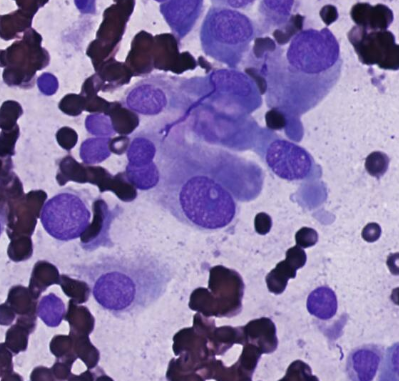
\includegraphics[scale=0.5]{image/inclusion_1.png}}
	\subfigure{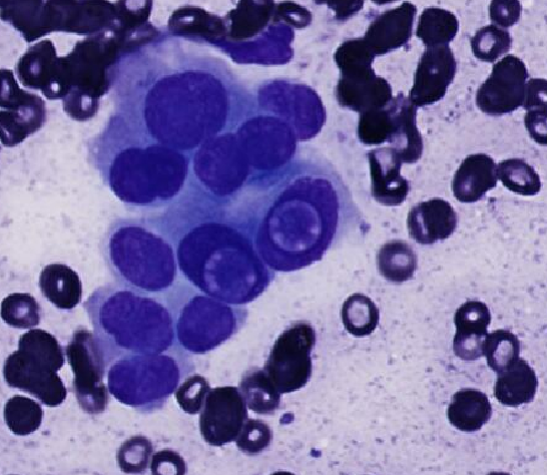
\includegraphics[scale=0.5]{image/inclusion_2.png}}
	\caption{Cells with inclusion}
	\label{fig:intro_inclu_ex}
\end{figure}

\begin{figure}
	\center
	\subfigure[Proliferative]{
		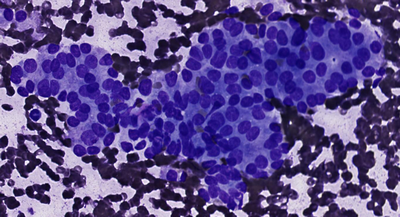
\includegraphics[scale=0.5]{image/prolif_pattern_1.png}
		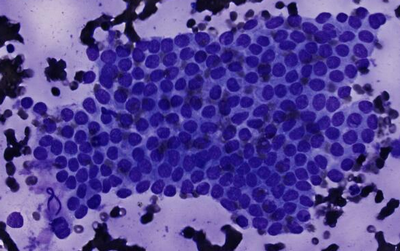
\includegraphics[scale=0.5]{image/prolif_pattern_2.png}
		\label{sfig:prolif_patterns}
	} \\
	\subfigure[Non-proliferative]{
		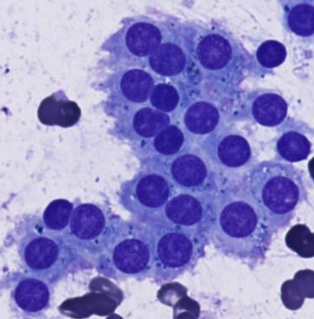
\includegraphics[scale=0.5]{image/normal_pattern_1.png}
		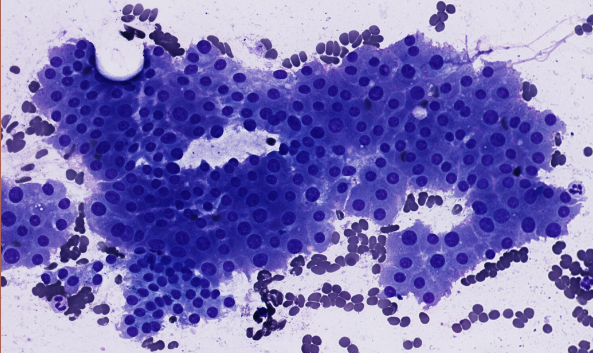
\includegraphics[scale=0.5]{image/normal_pattern_2.png}
		\label{sfig:norm_patterns}
	}
	\caption{Stained thyroid takings - architectural patterns}
	\label{fig:intro_pattern_ex}
\end{figure}

\subsubsection{Cytomine} 
Cytomine \cite{maree2016collaborative} is a web-based environment enabling collaborative multi-gigapixel image analysis. Users can navigate through those images, annotate them and associate domain specific labels to the generated annotations. The platform also integrates machine learning-based image recognition algorithms that can automatically produce annotations. A reviewing system enables experts to proofread those annotations. 

\subsubsection{Dataset}
\label{sssec:detection_thyroid_dataset}
A project dedicated to nodule malignancy detection was created on the Cytomine platform. It contains 61 annotated images with sizes ranging from 4 gigapixels to 18 gigapixels. Those images contain a total of 5784 labelled annotations performed by experts from the ULB (?? ref ??). Those labels (or terms) link the annotation to cytological objects related to the nodule malignancy problem. The terms made available on Cytomine are organized in an ontology which is divided into three main subcategories:

\begin{itemize}
	\item \textbf{Architectural patterns} : includes proliferative and non-proliferative patterns but also an intermediate class for patterns which present minor signs of proliferation.
	\item \textbf{Nuclear features} : includes cells with inclusion, normal cells and some additional cell-related terms
	\item \textbf{Others} : includes artefacts, background but also poly nuclear cells, red blood cells,...
\end{itemize} 

The complete ontology can be found in Appendix \ref{app:ontology}. Among those available terms, the ones that matter the most in the context of nodule malignancy detection are the cells with inclusion and the proliferative architectural patterns (major or with minor sign). Those terms represent the positive classes of the problem. The distributions of terms are given in Figure \ref{fig:ontology_histograms}. Those histograms highlight that a significant number of annotations have been made with the terms of interest. Moreover, the number of annotations is relatively balanced for those terms. While they are balanced taken alone, a problem arises when the terms are grouped. For instance, in the binary problem of determining whether a cell contains an inclusion or not, the positive class might be the term \textit{Cell with inclusion} while the negative class might contain the all the other terms from the cell subcategory (and possibly terms from the others subcategory). While being sound, this distribution of terms in both classes results in an imbalance which can be problematic when applying machine learning classification algorithms. The classes distribution for this example problem are given in Figure \ref{fig:imbalance_incl_vs_norm}.


\begin{figure}
	\center
	\subfigure[Main categories]{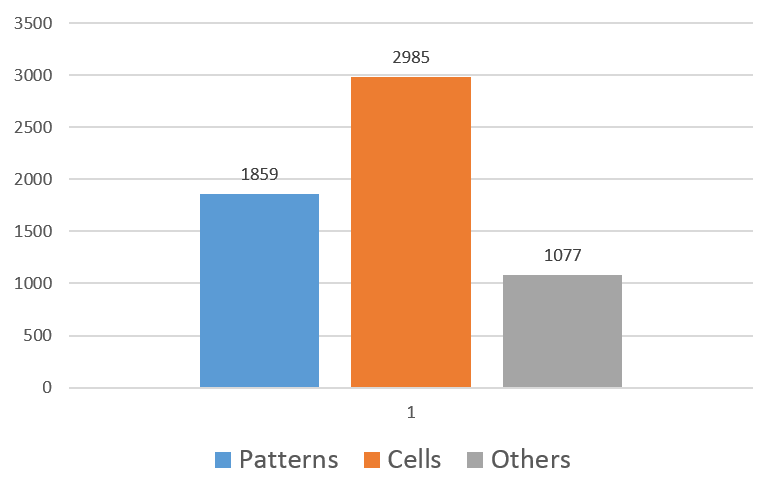
\includegraphics[scale=0.5]{image/ontology_hist_all.png}}
	\subfigure[Cell-related terms]{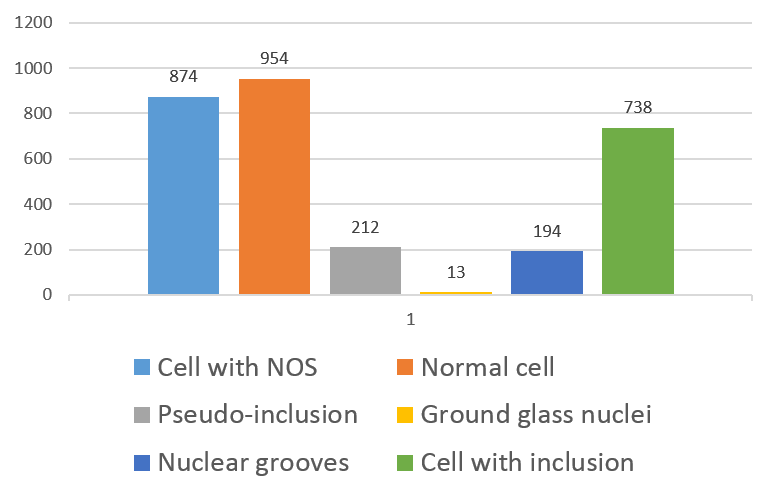
\includegraphics[scale=0.5]{image/ontology_hist_cells.png}}\\
	\subfigure[Pattern-related terms]{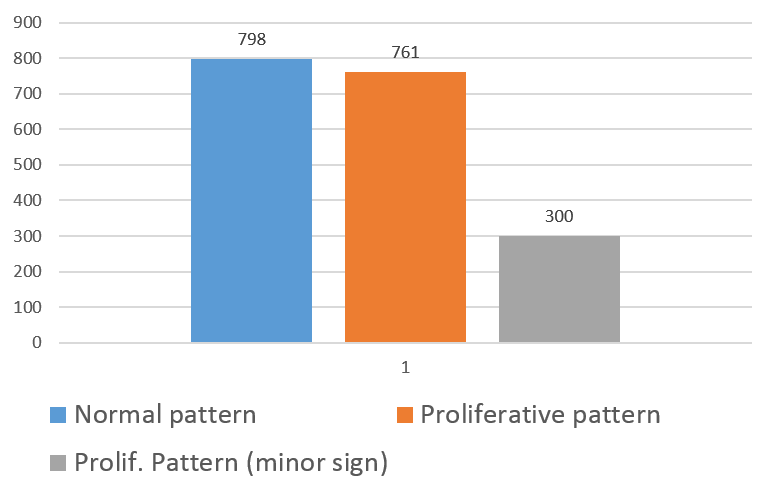
\includegraphics[scale=0.5]{image/ontology_hist_patterns.png}}
	\subfigure[Other terms]{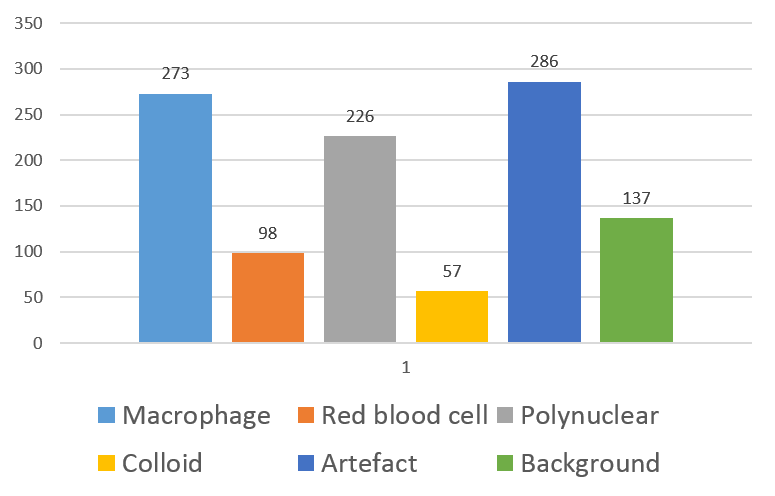
\includegraphics[scale=0.5]{image/ontology_hist_others.png}}
	\caption{Terms of the thyroid ontology - annotation counts histograms}
	\label{fig:ontology_histograms}
\end{figure}

\begin{figure}
	\center
	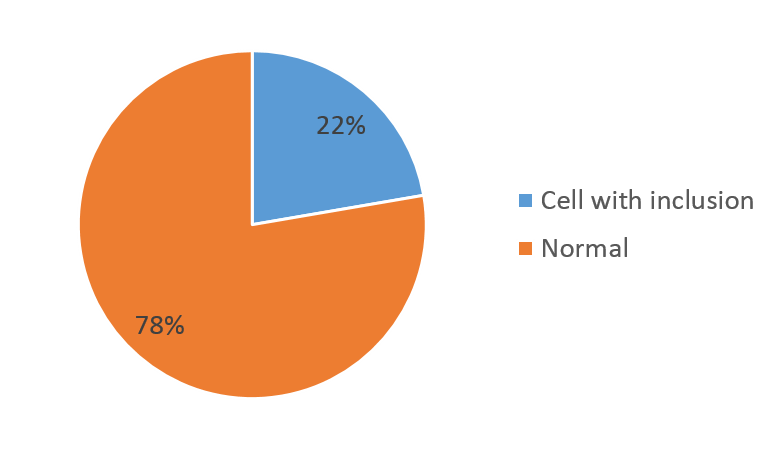
\includegraphics[scale=0.75]{image/imbalance_binary_problem.png}
	\caption{Cell inclusion detection problem. Terms in positive class: cell with inclusion. Terms in negative class: normal cells, pseudo inclusion, ground glass nuclei, nuclear grooves, red blood cells and poly-nuclear.}
	\label{fig:imbalance_incl_vs_norm}
\end{figure}